\section{Dispute Wheels and Dispute Rings}
\label{sec:dw}

Our goal is to study the classes of rankings for which the routing
system is guaranteed to be safe under filtering.  Griffin \ea have shown
that checking whether a particular 
routing system is safe is NP-hard \cite{Griffin2002c}.  To simplify our study of safety, we
introduce a useful concept developed by Griffin \ea \cite{Griffin2002c},
known as a {\em dispute wheel}.  Informally, a dispute wheel gives a
listing of 
nodes, and two path choices per node, such that one path is always
preferred to the other.  
%A fair activation sequence in which each node
%in the dispute wheel picks its more preferred path to its less preferred
%path leads to an oscillation.  
If a routing system oscillates, then it is possible to construct a
dispute wheel whereby each node in the wheel selects its more preferred
path (via the node in the clockwise direction) over its less preferred path.
Griffin \ea showed that if a
routing system with no filtering does not have a dispute wheel, then it
is safe. 

The dispute wheel is a useful concept because it allows us to analyze
dynamic properties such as safety by simply looking at the
rankings of each node in the routing system.  In this section, we formally
define a dispute wheel and show the relationship of Griffin's routing
model, which simulates messages being passed between nodes, to the model
we use in this chapter, which uses fair activation sequences.  This
relationship 
allows us to study safety in
terms of the routing model in this chapter.  We then introduce a special
type of dispute wheel 
called a {\em dispute ring} and show that, if any routing system has
a dispute ring, then it is not safe under filtering.  Finally, we relate
dispute wheels to dispute rings and show that, although the presence of
a dispute ring guarantees that a routing system is not safe under
filtering, it does not necessarily imply that a routing system is not safe
without filtering.  Figure~\ref{fig:stability_venn} summarizes the results of
this section and how they relate to results from previous
work~\cite{Griffin2002c}. 


\begin{figure}[t]
\centering
%\subfigure[Previous results.~\protect\cite{Griffin2002c}.]{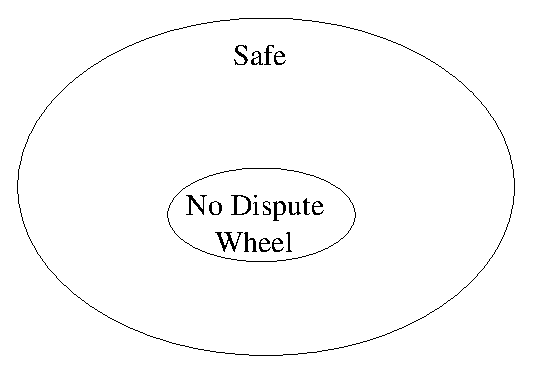
\epsfig{file=policy/figures/stability_venn_griffin.eps, width=0.43\columnwidth}}\hfill
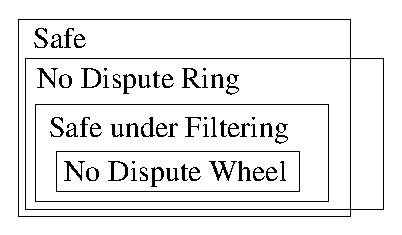
\epsfig{file=policy/figures/stability_venn.eps, width=0.5\columnwidth}
\caption[Relationships between safety and dispute rings and
  wheels.]{Relationships between safety and dispute rings and wheels. 
  Previous work showed that a routing system with no dispute wheel is
  safe~\protect\cite{Griffin2002c}.  Section~\ref{sec:dw} presents all other
  relationships shown in this figure.}
\label{fig:stability_venn}
\end{figure}



\subsection{Dispute Wheels and Safety}

%We start by formally defining dispute wheels.

\begin{defn}[Dispute wheel]
\label{def:dw}
Given a routing system $(N, \prec_1,\ldots, \prec_N, \F_1, \ldots,
\F_N)$, a {\em dispute wheel} is a collection of distinct nodes
$i_1, \ldots, i_m$, called {\em pivots}, together with two sets of
paths $P_1, \ldots, P_m$ and $Q_1, \ldots, Q_m$, such that the
following conditions all hold (where we define $i_{m+1} = i_1$ for
notational convenience):
\begin{enumerate}
\itemsep=-1pt
\item $P_{k} \in \F_{i_k}$ for all $k = 1,\ldots,m$;
\item $Q_{k}$ is a path from $i_k$ to $i_{k+1}$ for all $k =
1,\ldots,m$;
\item The path $\hat{P}_{k} = i_k Q_{k} i_{k+1} P_{k+1} 0$ is
feasible, \ie, $\hat{P}_{k} \in \F_{i_k}$,
% and 
\item $\hat{P}_{k} \succ_{i_k} i P_{k} 0$.
\end{enumerate}
\end{defn}
Thus, each node $i_k$ prefers the path $i_k Q_{k}i_{k+1}
P_{k+1} 0$ to the path $i_k P_{k} 0$, as shown in Figure~\ref{fig:dw}.




\begin{figure}
\centering
\begin{psfrags}
%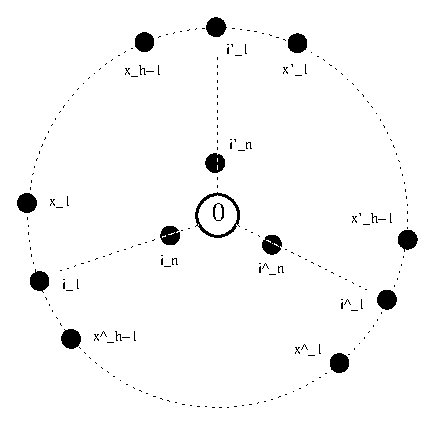
\epsfig{file=policy/figures/lemdr.eps,width=0.25\textwidth}
%
\psfrag{0}{{\Large $0$}}
\psfrag{Q_k}{{\Large $Q_k$}}
\psfrag{P_k}{{\Large $P_k$}}
\psfrag{i_k}{{\Large $i_k$}}
\psfrag{P_k+1}{{\Large $P_{k+1}$}}
\psfrag{i_k+1}{{\Large $i_{k+1}$}}
%
\resizebox{0.45\textwidth}{!}{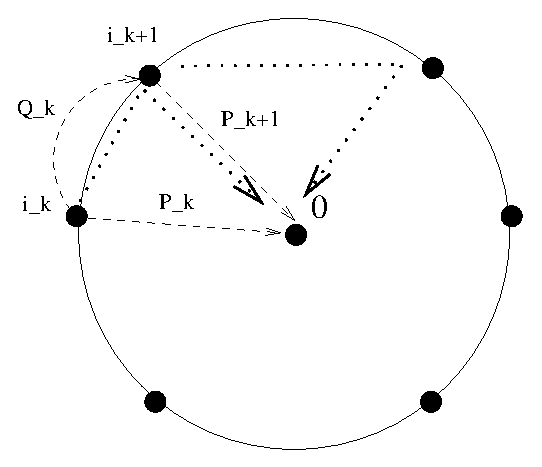
\includegraphics{policy/figures/dw.eps}}
\end{psfrags}
%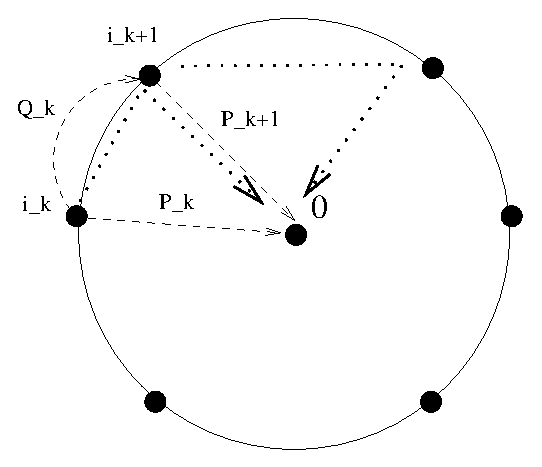
\epsfig{file=policy/figures/dw.eps,width=0.28\textwidth}
\caption[Illustration of a dispute wheel.]{Illustration of a dispute
  wheel.  Dotted lines show preferred 
  (indirect) paths to the destination.  The nodes $i_1, \ldots, i_m$
  are pivots.}
\label{fig:dw}
\end{figure}



%As previously shown by Griffin \ea\cite{Griffin2002c}, the most
%important feature of dispute wheels for our purposes is that if a
%routing system has no dispute wheels, then it is safe.  To use this
%result for analyzing routing systems as we defined in
%Definition~\ref{def:system} (Section~\ref{sec:notation}), 
We now show
  that safety in the Simple 
Path Vector Protocol (SPVP) defined by Griffin {\em et
al.}~\cite{Griffin2002c} implies safety in our model, which allows us to
  use dispute wheels to analyze safety. 

%% In previous work, Griffin defined a {\em simple path vector protocol
%% (SPVP)} as a model for BGP and showed that if a BGP system had no
%% dispute wheel, then SPVP was guaranteed to be safe for that BGP system
%% (\ie, convergent for all possible message orderings).  We show that if
%% the BGP system we have defined has no dispute wheel, then it is safe,
%% according to Definition~\ref{def:safety}, by showing the equivalence of
%% safety under SPVP to safety of the BGP system from
%% Definition~\ref{def:system}.  


\begin{prop}%[Griffin et al.~\cite{Griffin2002c}]
\label{prop:griffin}
Given a routing system, a fair activation sequence, and an initial
path assignment $\v{P}_0$, let $\v{P}_1, \v{P}_2, \ldots$ be the
resulting sequence of path assignments according to the dynamics
described in Figure \ref{fig:bgpdec}.  Then there exists a sequence of
messages in the Simple Path Vector Protocol (SPVP) such that the same
sequence of path assignments is observed.

Thus, in particular, if a routing system is safe under SPVP, then it is
safe according to Definition~\ref{def:safety}.
\end{prop}

\begin{proofsketch}
The key difference between SPVP and the dynamics we have defined is
that SPVP is {\em asynchronous} (\ie, at any time step, messages may
be in flight), so different nodes may have different assumptions about
the global path assignment at any time.  SPVP is {\em
nondeterministic} with respect to the timing of messages; the delay
between a routing update at node $j$ and the receipt of the new route
advertisement from node $j$ at node $i$ can be arbitrary.  We
use this fact to construct, inductively, a sequence of messages
such that at time $t$, the current set of paths available to node
$i_t$ in SPVP corresponds exactly to $\v{P}_{t-1}$.  Furthermore, we time
the delivery of routing updates to node $i_t$ in SPVP so that any
updates that occurred since the last time $i_t$ was activated arrive
exactly at the start of time step $t$.  In SPVP, this will initiate a
routing update at node $i_t$, which corresponds exactly to the
activation of $i_t$ in our model (see Figure~\ref{fig:bgpdec}).

Thus, the sequence of path assignments seen in this realization of SPVP
 matches the sequence of path assignments seen in our dynamics.  We
conclude that if SPVP is guaranteed to be safe for the
given routing system (\ie, if eventually no further routing updates
occur, regardless of the initial path assignment), then the routing
system is safe according to Definition \ref{def:safety} as well.
\end{proofsketch}

%\begin{corollary}
%If a routing system  $(N, \prec_1, \ldots,\prec_N,\lb \F_1, \ldots,
%\F_N)$ has no dispute wheel, then it is safe. 
%\end{corollary}

%\begin{proof}
%If a routing system has no dispute wheel, then
%SPVP is safe~\cite{Griffin2002c}.  By the preceding proposition,
%no dispute wheel implies safety in our model as well.
%\end{proof}

%%%%%%%%%%%%%%%%%%%%%%%%%%%%%%%%%%%%%%%%%%%%%%%%%%%%%%%%%%%%

%It is trivial to show a stronger fact: if no dispute wheel exists,
%then a routing system is actually safe under filtering.

\begin{corollary}
\label{cor:dwfilter}
If a routing system $(N, \prec_1,\ldots,\prec_N, \F_1, \ldots,
\F_N)$ has no dispute wheel, then it is safe under filtering (and
hence safe).
\end{corollary}

\begin{proof}
Choose subsets $\hat{\F}_i \subseteq \F_i$.  Then, any dispute wheel for
the routing system $\hat{S} = (N, \prec_1,\lb
\ldots, \prec_N, \hat{\F}_1, \ldots, \hat{\F}_N)$ is also a
dispute wheel for the original routing system $S = (N, \prec_1, \ldots,\lb
\prec_N, \F_1, \ldots, \F_N)$.  Thus, the result follows from
Proposition \ref{prop:griffin} and the results of \cite{Griffin2002c}.
%Thus, if no dispute wheel exists
%for the routing system $S$, then no dispute wheel exists for
%the routing system $\hat{S}$, and by
%Proposition \ref{prop:griffin} the system $\hat{S}$ is safe.  Thus, $S$
%is safe under filtering.
\end{proof}

If no dispute wheel exists, the routing system is safe under filtering,
but, unfortunately, this condition is not a 
necessary condition for safety, and thus not much can be said about a
system that does have a dispute wheel.  
%Griffin \ea showed
%that a system can be safe even if it does have a dispute wheel.
Furthermore, there exist routing systems that have a dispute wheel but
which are safe under filtering.

\begin{observation}
The existence of a dispute wheel does {\em not} imply that the routing
system is unsafe, nor that the routing system is not safe under
filtering.
\end{observation}


\begin{figure}
\centerline{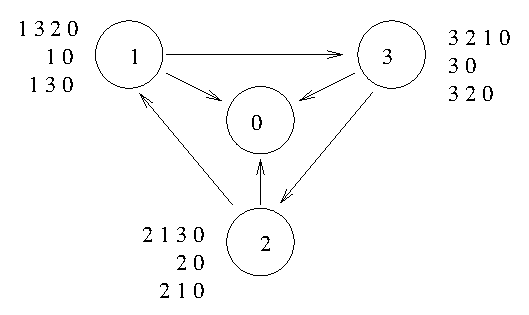
\epsfig{file=policy/figures/dw_no_osc.eps,width=0.5\textwidth}}
\caption{A routing system that is safe
  for any choice of filters.} 
\label{fig:dw_no_osc}
\end{figure}


\begin{example}
\label{ex:dw_no_osc}
See Figure~\ref{fig:dw_no_osc}.  The
first two most preferred paths in each node's ranking form
a dispute wheel, but the system is safe: the system converges to $\v{P}
= (10, 20, 30)$.  Furthermore, {\em no combination of filters can create an
oscillation}.  The two-hop paths are not part of the stable path
assignment, so filtering those paths has no effect on the protocol
dynamics.  Filtering a three-hop path would simply result in a node
selecting the direct path to the destination, and the node would never
deviate from that path.  If one
direct path is filtered, then the other two nodes will take direct paths
to the destination and the node whose direct path is filtered will take
its most preferred three-hop path.  If two direct paths are filtered,
then $\v{P}$ is simply a chain to the destination: the node that has the
direct path takes it, and the other two nodes will take two and
three-hop paths.
\end{example}

\subsection{Dispute Rings and Safety}

In this section, we extend the dispute wheel notion to understand the
relationship between ranking 
expressiveness and safety under filtering.  We define a relationship
between rankings called a {\em dispute ring}, a special case of a
dispute wheel where each node appears at most once.
The dispute ring is a useful concept because it allows us to prove a
{\em necessary} condition for safety under filtering.


\begin{defn}[Dispute ring]
\label{def:dr}
A {\em dispute ring} is a dispute wheel---a collection of nodes
$i_1, \ldots, i_m$ and paths $P_1, \ldots, P_m$, $Q_1, \ldots, Q_m$
satisfying Definition \ref{def:dw}---such that $m \geq 3$, and no node in
the routing system appears more than once in the wheel.
%% Formally, the following conditions must be 
%% satisfied for $k,\ell =1,\ldots, m$, such that $k \neq \ell$:
%% \begin{align*}
%% Q_{i_k} \cap Q_{i_\ell} & = \left\{ \begin{array}{ll}
%% i_\ell,& \textrm{if}\ \ell = k+1;\\
%% i_k,& \textrm{if}\ \ell=k-1;\\
%% \emptyset,& \textrm{otherwise};
%% \end{array}\right.\\
%% P_{i_k} \cap P_{i_\ell} & = \{0\}.
%% \end{align*}
%% In addition, the following conditions are satisfied for all $k,\ell
%% =1,\ldots, m$:
%% \[ Q_{i_k} \cap P_{i_\ell} = \left\{ \begin{array}{ll}
%% \emptyset,& \textrm{if}\ \ell \neq k;\\
%% i_k,& \textrm{if}\ \ell = k.
%% \end{array}\right. \]
\end{defn}

%% \begin{defn}
%% A {\em dispute ring} is a dispute wheel with the following property:
%% If $i_j \neq i_k$, then $P_{i_j} \cap P_{i_k} = \phi$, $Q_{i_j}
%% \cap Q_{i_k} = \phi$, $P_{i_j} \cap Q_{i_k} = \phi$, and $Q_{i_j} \cap
%% P_{i_k} = \phi$.  That is, a dispute ring is a dispute wheel for which
%% each node appears no more than once.
%% \end{defn}

%if a routing system has a
%dispute ring, then there exists some filtering configuration that will
%result in an oscillation (recall that the existence of a dispute wheel
%does not guarantee that the routing system will be unsafe, or even
%unsafe under filtering).  That is, there exists some choice of filters
%for which the routing system is unsafe.

\begin{prop}
\label{prop:drsafety}
If a routing system has a dispute ring, then it is not safe under filtering.
\end{prop}

\begin{proof}
Assume that a routing system has a dispute ring, defined by $i_1,
\ldots, i_m$, and paths $Q_1,\ldots, Q_m$, $P_1,\ldots, P_m$.  Then, construct
filters such that $\F_i$ contains {\em only} the paths in that
dispute ring.  Specifically, $\F_i$ contains the following paths
from $\P_i^N$ (where we define $i_{m+1} = i_1$).
%\begin{itemize}
%\itemsep=-1pt
(1) If $i$ is not in the dispute ring, then $\F_i = \emptyset$.
(2) If $i$ is a pivot node on the dispute ring, say $i = i_k$, then $\F_i$ contains
  exactly two paths: $P_k$, and $i_k Q_k i_{k+1} P_{k+1}
0$.
(3) If $i$ is not a pivot node, but $i \in Q_k$ for some $k$,
then we can write $Q_k = i_k Q_k^1 i Q_k^2 i_{k+1}$.  In this case
$\F_i$ consists of the single path $i Q_k^2 i_{k+1} P_{k+1} 0$.
(4) If $i$ is not a pivot node, but $i\in P_k$ for some $k$, then we
can write $P_k = i_k P_k^1 i P_k^2 0$.  In this case, $\F_i$ consists
  of the   single path $i P_k^2 0$.
%\end{itemize}
Since each node appears at most once on the dispute ring, the
preceding definition uniquely defines $\F_i$ for all nodes $i$.

There exists at least one consistent path assignment $\v{P}_t$ such
that some pivot node $i_{k-1}$ uses its most preferred path,
$i_{k-1} Q_{k-1} i_k P_{k} 0$, every other pivot node $i_j$ uses
path $i_j P_{j} 0$, and every other non-pivot node $i$ uses
its only available path consistent with this assignment.  Then, the
following activation sequence will result in an oscillation:
\begin{enumerate}
\itemsep=-1pt
\item {\em Activate node $i_k$.}  Node $i_k$ then switches to its more
  preferred path, $i_k Q_{k} i_{k+1} P_{k+1} 0$.  
\item {\em Activate nodes along $Q_{k-1}$ in reverse order, from
the node immediately preceding $i_{k}$, to $i_{k-1}$.}  All nodes
  along $Q_{k-1}$ switch to the empty path, $\epsilon$.
\item {\em Activate node $i_{k-1}$.}  The path $i_{k-1} Q_{k-1} i_k P_{k}
  0$ is now inconsistent, so $i_{k-1}$ must switch to the path $i_{k-1} P_{k-1} 0$.
\item {\em Return to Step~1 with $k$ replaced by $k+1$, and iterate again.}
\end{enumerate}
By the fourth step of the iteration above, the new path assignment is
``isomorphic'' to the initial configuration: now node $i_k$ is using
the path $i_k Q_k i_{k+1} P_{k+1} 0$, and every other pivot node $i_j$ is
using path $i_j P_j 0$.  Thus, as this iteration repeats, the
dynamics will ultimately reach node $i_k$ once again with the
original path assignment.  Note that all paths in this activation
sequence are guaranteed to be available and consistent, by the
definition of $\F_i$.
%, since $P_{i_j} \cap P_{i_k} = \phi$, $Q_{i_j} \cap Q_{i_k} =
%\phi$, $P_{i_j} \cap Q_{i_k} = \phi$, and $Q_{i_j} \cap P_{i_k} = \phi$.
%
To make this activation sequence fair, we must also activate the
nodes that are not in $P_{i} \cup Q_{i}$ for any $i$ in the dispute
ring; and the non-pivot nodes in $P_i$ for all $i$ in the dispute ring.  The
nodes that are not in $P_{i} \cup Q_{i}$ for any $i$ have only the path
$\epsilon$ available, and each non-pivot node in $P_i$ (for all $i$) has
only one 
path to the destination available. Therefore, these nodes will never
change paths, and do not affect the oscillation.
\end{proof}

We emphasize that, for simplicity, we reduced the set of filters,
$\F_i$, to include 
only the set of paths that are involved in an oscillation.  We note
that there will typically be more permissive sets $\F_i$ that will
also result in oscillation, because the dispute ring is present in the
underlying set of rankings.  Our intent is to highlight the
most basic case of filtering that can cause an oscillation, given the
existence of a dispute ring.


\begin{figure}[t]
\centering
\subfigure[Routing system]{
%{\scriptsize
\parbox{0.4\linewidth}{
\vspace*{-1.5in}
\hspace*{0.5in}
\begin{tabular}{l|l}
{\em Node} & {\em Ranking} \\ \hline
1 & $160 \succ 1240$ \\
2 & $240 \succ 2350$ \\
3 & $350 \succ 3160$ \\
4 & $43160 \succ 40$ \\
5 & $51240 \succ 50$ \\
6 & $62350 \succ 60$
\end{tabular}
%}
}} \hfill
%
\subfigure[Dispute wheel]{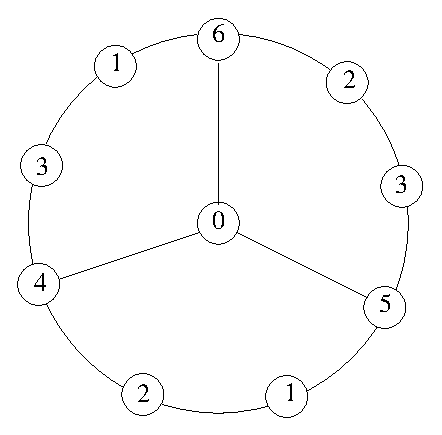
\epsfig{file=policy/figures/no_osc.eps,width=0.45\linewidth}}
\caption[Routing system that has no dispute ring and is not
  safe.]{System that (1)~has no dispute ring and (2)~is not safe.} 
\label{fig:wheel_no_ring}
\end{figure}

\begin{figure}[t]
%{\scriptsize
\begin{center}
\begin{tabular}{l|cccccc}
& \multicolumn{6}{c}{{\em Path Assignment}}  \\
{\em Act.} & 1 & 2 & 3 & 4 & 5 & 6\\ \hline
%% --- & (1 2 4 0) & (2 4 0) & (3 5 0) & (4 0) & (5 0) & (6 0) \\ 
%% 5 &   & & & & {\bf (5 1 2 4 0)} & \\ 
%% 1 &  {\bf (1 6 0)} & & & & & \\ 
%% 3 &   & & {\bf (3 1 6 0)} & & & \\ 
%% 4 &  & & & {\bf (4 3 1 6 0)} & & \\  
%% 5 &  & & & & {\bf (5 0)} & \\ 
%% 3 &  & & {\bf (3 5 0)} & & & \\ 
%% 2 &  & {\bf (2 3 5 0)} & & & &
%% \\ 
%% 6 &  & & & & & {\bf (6 2 3 5 0)} \\ 
%% 4 &  & & & {\bf (4 0)} & & \\ 
%% 2 &   & {\bf (2 4 0)} & & & & \\ 
%% 1 &  {\bf (1 2 4 0)} & & & & & \\ 
%% 5 &   & & & & {\bf (5 1 2 4 0)} & \\  
%% 6 &  & & & & & {\bf (6 0)} \\   

--- & (1 2 4 0) & (2 4 0) & (3 5 0) & (4 0) & (5 0) & (6 0) \\ 
5 &  (1 2 4 0) & (2 4 0) & (3 5 0) & (4 0) & {\bf (5 1 2 4 0)} & (6 0)
\\ 
1 &  {\bf (1 6 0)} & (2 4 0) & (3 5 0) & (4 0) & (5 1 2 4 0) & (6 0) \\ 
3 &  (1 6 0) & (2 4 0) & {\bf (3 1 6 0)} & (4 0) & (5 1 2 4 0) & (6 0)
\\ 
4 &  (1 6 0) & (2 4 0) & (3 1 6 0) & {\bf (4 3 1 6 0)} & (5 1 2 4 0) &
(6 0) \\  
5 &  (1 6 0) & (2 4 0) & (3 1 6 0) & (4 3 1 6 0) & {\bf (5 0)} & (6 0) \\ 
3 &  (1 6 0) & (2 4 0) & {\bf (3 5 0)} & (4 3 1 6 0) & (5 0) & (6 0) \\ 
2 &  (1 6 0) & {\bf (2 3 5 0)} & (3 5 0) & (4 3 1 6 0) & (5 0) & (6 0)
\\ 
6 &  (1 6 0) & (2 3 5 0) & (3 5 0) & (4 3 1 6 0) & (5 0) & {\bf (6 2 3 5
  0)} \\ 
4 &  (1 6 0) & (2 3 5 0) & (3 5 0) & {\bf (4 0)} & (5 0) & (6 2 3 5 0)
\\ 
2 &  (1 6 0) & {\bf (2 4 0)} & (3 5 0) & (4 0) & (5 0) & (6 2 3 5 0) \\ 
1 &  {\bf (1 2 4 0)} & (2 4 0) & (3 5 0) & (4 0) & (5 0) & (6 2 3 5 0)
\\ 
5 &  (1 2 4 0) & (2 4 0) & (3 5 0) & (4 0) & {\bf (5 1 2 4 0)} & (6 2 3
5 0) \\  
6 &  (1 2 4 0) & (2 4 0) & (3 5 0) & (4 0) & (5 1 2 4 0) & {\bf (6
  0)} \\   
\end{tabular}
\end{center}
%}
\caption{Activation sequence for unsafe system from
  Figure~\ref{fig:wheel_no_ring}.}  
\label{fig:wheel_no_ring_activation}
\end{figure}



Despite the fact that systems that are safe under filtering are
guaranteed not to have a dispute ring, testing for a dispute ring is
not sufficient to guarantee that the routing system is safe, because of
the following observation
%as there
%exist routing systems without dispute rings that are unsafe.  We give an
%example below.


\begin{observation}
Routing systems that have a dispute wheel but do not
have a dispute ring may not be safe. 
\end{observation}




\begin{example}
Consider the routing system described by Figure~\ref{fig:wheel_no_ring}(a)
and the corresponding dispute wheel in Figure~\ref{fig:wheel_no_ring}(b).
Suppose that nodes $1$, $2$, and $3$ prefer two-hop paths over
three-hop paths, and the only paths available to nodes are those depicted
in the figure.  This system is not safe; for
example, suppose $\v{P}_0 = (1240, 240, 350, 40, 50, 60)$.  The system
then oscillates as shown in Figure~\ref{fig:wheel_no_ring_activation}.
However, the system has no dispute ring; in particular, the dispute
wheel depicted in 
Figure~\ref{fig:wheel_no_ring}(b) cannot be reduced to a dispute ring.
\end{example}




